\documentclass[10pt]{beamer}

\usetheme{metropolis}
\usepackage{appendixnumberbeamer}

\usepackage{booktabs}
\usepackage[scale=2]{ccicons}

\usepackage{pgfplots}
\usepgfplotslibrary{dateplot}

\usepackage{xspace}
\newcommand{\themename}{\textbf{\textsc{metropolis}}\xspace}

\usepackage[utf8]{inputenc}
\usepackage[T1]{fontenc}

\usepackage{listings}
\usepackage{xcolor}
\lstdefinestyle{sharpc}{language=[Sharp]C, frame=lr, rulecolor=\color{blue!80!black}}


\title{Programação Assíncrona e Paralelismo}
\subtitle{Techtalk TODO: Pesquisar AKKA}
%\date{\today}
\author{Johnathan Fercher}
%\institute{Braspag}
% \titlegraphic{\hfill
\includegraphics[height=1.5cm]{logo.pdf}}

\begin{document}
\maketitle

\begin{frame}{Table of contents}
  \setbeamertemplate{section in toc}[sections numbered]
  \tableofcontents[hideallsubsections]
\end{frame}

\section{Introdução}

\begin{frame}[fragile]{Definições}

  \textbf{Programação Assíncrona} tem o propósito de possibilitar a execução de tarefas demoradas sem o bloqueio da execução.

  \textbf{Programação Paralela} tem o propósito de possibilitar a execução de tarefas ao mesmo tempo.
  
\end{frame}
\begin{frame}[fragile]{Problema assíncrono}
	\begin{itemize}
		\item Consumir uma API;
		\item Operações de CRUD em banco de dados;
		\item Quaisquer outras operações que demorem: \textbf{Treinamento de Inteligências Artificiais, Processamento de Imagens e Etc};
	\end{itemize}
\end{frame}

\begin{frame}[fragile]{Problema paralelo}
	\begin{itemize}
		\item \textbf{Em um jogo:} Uma thread é responsável por obter os comandos do Joystick e outras $N$ são responsáveis por controlar a renderização de objetos, comandos de adversários e etc;
		\item \textbf{Em um robô}: Uma thread é responsável pela leitura de sensores e outras $N$ são responsáveis por controlar motores, realizar comunicação com outros robôs e etc;
		\item \textbf{Em um algoritmo de reconhecimento facial:} Pode-se dividir uma imagem em quadrantes, onde N threads serão responsáveis por aplicar filtros nas secções;
	\end{itemize}
\end{frame}

\section{Programação Síncrona e Assíncrona em C\#}

\begin{frame}{Simples código síncrono}
	\textbf{exemplo}
\end{frame}

\begin{frame}{Simples código assíncrono}
	\textbf{exemplo}
\end{frame}

\begin{frame}{Transformando código síncronos em assíncronos}
	\textbf{exemplo}
\end{frame}

\begin{frame}{Transformando código assíncronos em síncronos}
	\textbf{exemplo}
\end{frame}

\begin{frame}{Exemplos para Benchmark}
	\textbf{Sync x Async}
\end{frame}


\begin{frame}{Benchmark}
	\begin{figure}
		\begin{tikzpicture}
		\begin{axis}[
		mbarplot,
		ymin=0, ymax=5.5,
		%xlabel={Foo},
		ylabel={Tempo de Execução},
		width=0.9\textwidth,
		height=6cm,
		xticklabels={,,}
		]
		
		\addplot plot coordinates {(0, 5.33539)};
		\addplot plot coordinates {(0, 5.35828)};
		
		\legend{Sync (5.33539s), Async (5.35828s)}
		
		\end{axis}
		\end{tikzpicture}
	\end{figure}
\end{frame}

\begin{frame}{Fui tapeado?}
	\begin{alertblock}{Por que não houve ganhos de performance?}
		Programação Assíncrona apenas é responsável por não bloquear a execução.
	\end{alertblock}
	\begin{exampleblock}{Então para que vou usar isso?}
		Depende da aplicação.
	\end{exampleblock}
\end{frame}

\begin{frame}{Vantagens da Programação Assíncrona}
	\begin{itemize}
		\item \textbf{Em aplicações que possuem front-end}: A principal vantagem é o aprimoramento da interação com a aplicação; 
		\item \textbf{Em um servidor}: A principal vantagem é o aprimoramento da escalabilidade;
	\end{itemize}
\end{frame}

\begin{frame}{Uma requisição síncrona no WebAPI}
	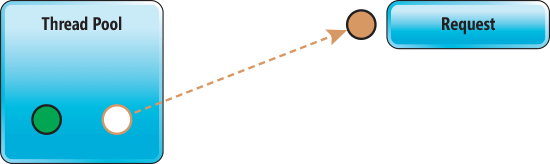
\includegraphics[width=\textwidth]{imgs/sync1}
	\begin{itemize}
		\item Uma thread livre e outra thread bloqueada realizando \textbf{nada};
	\end{itemize}
\end{frame}

\begin{frame}{Três requisições síncronas no WebAPI}
	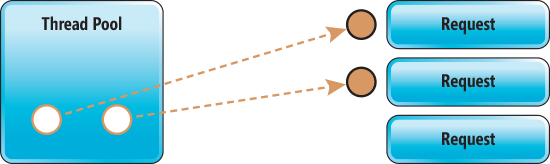
\includegraphics[width=\textwidth]{imgs/sync2}
	\begin{itemize}
		\item Duas threads bloqueadas realizando \textbf{nada} e uma requisição em espera;
	\end{itemize}
\end{frame}

\begin{frame}{Uma requisição assíncrona no WebAPI}
	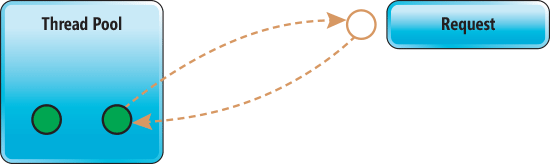
\includegraphics[width=\textwidth]{imgs/async}
	\begin{itemize}
		\item Thread realiza uma requisição bloqueante e retorna para a espera;
	\end{itemize}
\end{frame}

\begin{frame}{Ganhos}
	\vspace{0.5cm}
	Redução de custos em relação à memória e redução do tempo de CPU desperdiçado; 
\end{frame}

\section{Paralelismo em C\#}

\begin{frame}{Exemplo para Benchmark}
	\textbf{SyncDataParallel}
\end{frame}

\begin{frame}{Benchmark}
	\begin{figure}
		\begin{tikzpicture}
		\begin{axis}[
		mbarplot,
		ymin=0, ymax=5.5,
		%xlabel={Foo},
		ylabel={Tempo de Execução},
		width=0.9\textwidth,
		height=6cm,
		xticklabels={,,}
		]
		
		\addplot plot coordinates {(0, 5.33539)};
		\addplot plot coordinates {(0, 5.35828)};
		\addplot plot coordinates {(0, 3.62243)};
		
		\legend{Sync (5.33s), Async (5.35s), SyncD (3.62s)}
		
		\end{axis}
		\end{tikzpicture}
	\end{figure}
\end{frame}


\begin{frame}{Perguntas Frequentes}
	\begin{exampleblock}{Posso aplicar isso em qualquer problema?}
		Depende da quantidade de transformação de dados envolvida.
	\end{exampleblock}
	\begin{exampleblock}{Quanto maior o número de threads melhor?}
		Existe um limiar onde a aplicação gasta mais tempo na comunicação entre threads do que o ganho de performance na execução paralela.
	\end{exampleblock}
\end{frame}

\begin{frame}{Tipos de Paralelismo}
	Paralelismo de Tarefas
	
	Paralelismo de Dados
\end{frame}

\begin{frame}{Exemplo para Benchmark}
	\textbf{AsyncTaskParallel}
\end{frame}

\begin{frame}{Benchmark}
	\begin{figure}
		\begin{tikzpicture}
		\begin{axis}[
		mbarplot,
		ymin=0, ymax=5.5,
		%xlabel={Foo},
		ylabel={Tempo de Execução},
		width=0.9\textwidth,
		height=6cm,
		xticklabels={,,}
		]
		
		\addplot plot coordinates {(0, 5.33539)};
		\addplot plot coordinates {(0, 5.35828)};
		\addplot plot coordinates {(0, 3.62243)};
		\addplot plot coordinates {(0, 4.85521)};
		
		\legend{Sync (5.33s), Async (5.35s), SyncD (3.62s), AsyncT (4.85s)}
		
		\end{axis}
		\end{tikzpicture}
	\end{figure}
\end{frame}

\begin{frame}{Exemplo para Benchmark}
	\textbf{AsyncTaskAndDataParallel}
\end{frame}

\begin{frame}{Benchmark}
	\begin{figure}
		\begin{tikzpicture}
		\begin{axis}[
		mbarplot,
		ymin=0, ymax=5.5,
		%xlabel={Foo},
		ylabel={Tempo de Execução},
		width=0.9\textwidth,
		height=6cm,
		xticklabels={,,}
		]
		
		\addplot plot coordinates {(0, 5.33539)};
		\addplot plot coordinates {(0, 5.35828)};
		\addplot plot coordinates {(0, 3.62243)};
		\addplot plot coordinates {(0, 4.85521)};
		\addplot plot coordinates {(0, 3.18459)};
		
		\legend{Sync (5.33s), Async (5.35s), SyncD (3.62s), AsyncT (4.85s), AsyncDT (3.18s)}
		
		\end{axis}
		\end{tikzpicture}
	\end{figure}
\end{frame}

\begin{frame}{Exemplo para Benchmark}
	\textbf{AsyncTaskAndDataParallel}
\end{frame}

\begin{frame}{Benchmark}
	\begin{figure}
		\begin{tikzpicture}
		\begin{axis}[
		mbarplot,
		ymin=0, ymax=5.5,
		%xlabel={Foo},
		ylabel={Tempo de Execução},
		width=0.9\textwidth,
		height=6cm,
		xticklabels={,,}
		]
		
		\addplot plot coordinates {(0, 5.33539)};
		\addplot plot coordinates {(0, 5.35828)};
		\addplot plot coordinates {(0, 3.62243)};
		\addplot plot coordinates {(0, 4.85521)};
		\addplot plot coordinates {(0, 3.18459)};
		\addplot plot coordinates {(0, 2.68165)};
		
		\legend{Sync (5.33s), Async (5.35s), SyncD (3.62s), AsyncT (4.85s), AsyncDT (3.18s), AsyncDTFF (2.68s)}
		
		\end{axis}
		\end{tikzpicture}
	\end{figure}
\end{frame}

\begin{frame}{Problemas de Paralelismo}
	\begin{itemize}
		\item Execução em ordem imprevisível;
		\item Condição de corrida;
		\item Execuções problemáticas;
		\item Falhas e Exceções;
	\end{itemize}
\end{frame}

\begin{frame}{Técnicas para evitar problemas}
	\begin{itemize}
		\item Lock;
		\item Mutex;
		\item Semáforos;
		\item Monitor;
		\item Passagem de Mensagens;
	\end{itemize}
\end{frame}

\begin{frame}{Técnicas para evitar problemas}
	\begin{itemize}
		\item Mestre e Escravo;
		\item Escritor e Leitores;
		\item 3 Monges;
		\end{itemize}
\end{frame}

\begin{frame}[standout]
  Perguntas?
\end{frame}

\end{document}
